
%%%%%%%%%%%%%%%%%%%%%%% file typeinst.tex %%%%%%%%%%%%%%%%%%%%%%%%%
%
% This is the LaTeX source for the instructions to authors using
% the LaTeX document class 'llncs.cls' for contributions to
% the Lecture Notes in Computer Sciences series.
% http://www.springer.com/lncs       Springer Heidelberg 2006/05/04
%
% It may be used as a template for your own input - copy it
% to a new file with a new name and use it as the basis
% for your article.
%
% NB: the document class 'llncs' has its own and detailed documentation, see
% ftp://ftp.springer.de/data/pubftp/pub/tex/latex/llncs/latex2e/llncsdoc.pdf
%
%%%%%%%%%%%%%%%%%%%%%%%%%%%%%%%%%%%%%%%%%%%%%%%%%%%%%%%%%%%%%%%%%%%


\documentclass[runningheads,a4paper]{llncs}
\usepackage[a4paper, total={6in, 8in}]{geometry}
\usepackage{amssymb}
\setcounter{tocdepth}{3}
\usepackage{graphicx}
\usepackage{subcaption}
\usepackage{listings}
%\lstset{
%	numbers=left
%	language=Java
%	frame=single,
%	breaklines=true,
	%postbreak=\raisebox{0ex}[0ex][0ex]{\ensuremath{\color{red}\hookrightarrow\space}}
%}
\renewcommand{\lstlistingname}{Code}

\captionsetup{compatibility=false}

\usepackage{url}
\urldef{\mailsa}\path|{alfred.hofmann, ursula.barth, ingrid.haas, frank.holzwarth,|
\urldef{\mailsb}\path|anna.kramer, leonie.kunz, christine.reiss, nicole.sator,|
\urldef{\mailsc}\path|erika.siebert-cole, peter.strasser, lncs}@springer.com|    
\newcommand{\keywords}[1]{\par\addvspace\baselineskip
\noindent\keywordname\enspace\ignorespaces#1}

\begin{document}

\mainmatter  


\newpage
\tableofcontents
\newpage

\abstract{
The implementation of parallel computing the integral of a function from Monte Carlo method is described in this assignment.
Particularly, the assignment exploits the FastFlow parallel framework and C++ threads for building stream parallelism including pipeline and farm.
The experiments illustrate the comparison of time consuming of these ways.
} 

\section{Introduction}
\label{sec:intro}
% Describe that dataset and generally about sections


With the development of hardware technologies and a plenty of data, the requirement of time consuming to process or compute some tasks have been noticed.
Therefore, the parallelism is considered and utilized. The parallelism tasks are divided into some parts such as: stream parallelism, data parallelism, task parallelism and so on.

This assignment is about exploiting the stream parallelism on computing integral of a given function with Monte Carlo method.
Because of a stream of interval numbers from the requirement of the project, the stream parallelism with pipeline and farm is utilized to parallel computing the Monte Carlo method for each interval number.
To create a stream parallelism structure, the FastFlow (FF) framework and C++ threads are mentioned in this assignment.


The remaining of the assignment is constructed: the Section~\ref{sec:imple} describes about the implementation of computing the integral of a given function with Monte Carlo. 
The results and experiments using FF and C++ threads are represented in Section~\ref{sec:exper}, while Section~\ref{Conc} concludes the assignment.
	
\section{Implementation}
\label{sec:imple}

In this part of the report, the general idea of the Monte Carlo in computation of a integral function is design with FF and C++ threads.
The basic idea is about forming an interval number object with basic fields and methods. Hence, each interval number goes through each stage which executes specific tasks in stream parallelism built by FF and C++ threads.

\subsection{FastFlow}
\label{subsec:ff}

\begin{figure*}[h!]
	\centering
	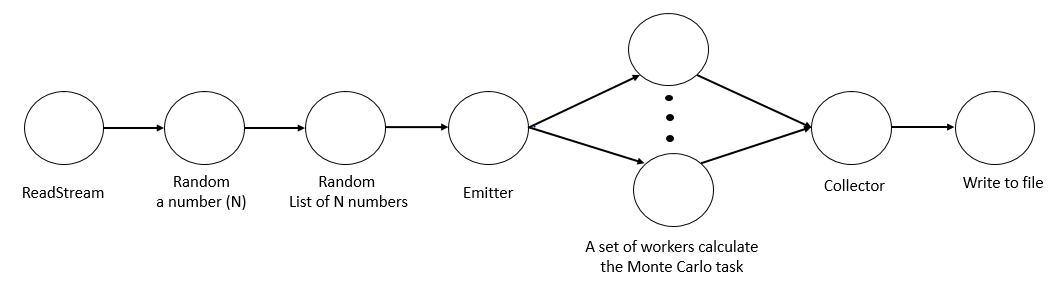
\includegraphics[scale = 0.4]{image/ffStructure}	
	\caption{The diagram of FF structure}
	\label{Fig:ffStructure}
\end{figure*}

To build a parallelism of the Monte Carlo method for computing integral of a function, the FF a structured parallel programming framework is utilized because of plenty of advantages such as highly efficient stream parallel and a set of ready-to-use for programmers.
In addition, FF can be flexible for creation complex parallelism with a lot of different nodes.


With the Monte Carlo task, the FF framework is used to build a structure stream parallelism with pipeline and farm.
Particularly, from the Fig~\ref{Fig:ffStructure}, it can be clear that the structure is built based on a set of stages including:
reading a set of interval numbers, choosing a random number (N), choosing a list of N numbers, setting Monte Carlo number calculations to threads and writing to a file.

Generally, each stage has a specific task to resolve. 
Because of the convenience of FF, each of stage or task or node is implemented as a function. 
However, if the a stage has more than one input or out put, it can be redefined.
In more detail, the tasks of stages is described:
\begin{itemize}
\item readStream: takes a couple numbers at each time from a stream of file.
\item random a number (N): randomly selects a number.
\item random a list of N numbers: is generated from this stages.
\item emitter: split interval numbers to free workers.
\item a set of workers: compute Monte Carlo method for set of interval numbers.
\item collector: takes bunch of interval numbers and send to the next stage.
\item write to file: write the Monte Carlo to a file.
\end{itemize}

\subsection{C++ Thread}
\label{subsec:thread}

\begin{figure*}[h!]
	\centering
	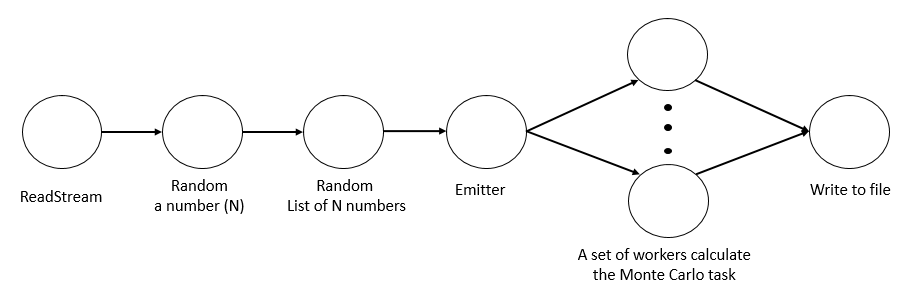
\includegraphics[scale = 0.4]{image/threadStructure}	
	\caption{The diagram of C++ threads structure}
	\label{Fig:threadStructure}
\end{figure*}

In case of using C++ threads, the similar construction is built with pipeline and farm on stream parallelism (in the Fig~\ref{Fig:threadStructure}). 
However, without supporting from FF, the communication between stages is executed through queues and combination of mutex and condition variable in C++.
In more detail, the queues run a role like containers which hold interval numbers executed from previous stage and waiting the next call of the next stage.
Meanwhile, the mutex and condition variable are similar to doors and bells, respectively.
Particularly, to start a stage by a thread, the mutex is used to lock the thread.
After a stage has completed its task, the thread is unlocked by the mutex and sends a notify to next threads waiting for their turns.
Based on some conditions, the notified threads can be waken up for their tasks or still sleep.
In addition, each stage in case of C++ threads is implemented by a thread with a specific task like FF construction.
The idea of stream parallelism in C++ threads construction is also similar the way of FF construction. 
Nevertheless, at the last stage, the C++ threads construction uses a queue to contain results of workers, in stead of using a collector to gather output of workers from farm.
Then the final stage pops each result from queue to a file.


%Each of the output of stage or thread is a queue from which the next stage can take sequential objects to compute.
%However, it exists some problems in case of race condition.
%Therefore, the mutex ... and condition variable techniques are utilized to lock and unlock some data.
%In case of using C++ threads implementing this task, 
%For a parallelism 
%http://www.cplusplus.com/reference/thread/thread/
%threads ....
%condition variable 
%mutex...


\section{Experiments}
\label{sec:exper}
The experiments of the Monte Carlo task with FF framework and C++ threads are mentioned in this section.
Particularly, a set of different functions is tried with different of power. However, a fixed of interval numbers is considered with ... couples.

\subsection{FastFlow}

\subsection{C++ thread}


\section{Conclusion}
\label{Conc}
The computation of integral of a given function with Monte Carlo method is implemented with stream parallelism.
In more detail, the implementation is built based on the combination of pipeline and farm with FF framework and C++ threads.
The comparison of these techniques are

\section{Ackowledgements}
I would like to show my gratitude to Prof. Marco Danelutto and his Assistant Dr. Massimo Torquati about lessons in Distributed systems: paradigms and models course at University of Pisa.
Additionally, I say thank to my friends who support and encourage me in this course.

\bibliography{Ref}
\bibliographystyle{plain}

\end{document}

\iffals

\section{Metrics and Activation}
\label{Metrics}
\subsection{Sigmoid}
\subsection{Activation Function}
\subsection{Identity Function}
\subsection{UnitStep}
\section{Cross-Validation}
\label{CV}



\begin{figure*}[t!]
	\centering
	\begin{subfigure}[b]{0.6\textwidth}
		%\centering
		
\includegraphics[scale = 0.6]{image/Unipi_Image}
		\caption{In-degree distribution with an exponent 4.5}
	\end{subfigure}
	\\
	\begin{subfigure}[b]{0.6\textwidth}
		%\centering
		
\includegraphics[scale = 0.6]{image/Unipi_Image}
		\caption{Out-degree distribution with an exponent 5.5}
	\end{subfigure}
	\caption{In-degree and Out-degree distributions}
		\label{Fig:Distri}
\end{figure*}
\textbf{Second Part}:
\begin{figure*}[t!]
	\centering
	\begin{subfigure}[b]{0.6\textwidth}
		%\centering
		
\includegraphics[scale = 0.6]{image/Unipi_Image}
		\caption{Size of WCC distribution with an exponent 10 of power law}
	\end{subfigure}
	\\
	\begin{subfigure}[b]{0.6\textwidth}
		%\centering
		
\includegraphics[scale = 0.6]{image/Unipi_Image}
		\caption{Size of SCC distribution with an exponent 9 of power law}
	\end{subfigure}

	\caption{Size of WCC and SCC distributions}
		\label{Fig:WCC_SCC}
\end{figure*}

\begin{figure*}[t!]

	\centering
	\begin{subfigure}[b]{0.6\textwidth}
		%\centering
		
\includegraphics[scale = 0.6]{image/Unipi_Image}
		\caption{Experiment with BFS on forward direction}
	\end{subfigure}
	\\
	\begin{subfigure}[b]{0.6\textwidth}
		%\centering
		
\includegraphics[scale = 0.6]{image/Unipi_Image}
		\caption{Experiment with BFS on backward direction}
	\end{subfigure}
	\\
	\begin{subfigure}[b]{0.6\textwidth}
		%\centering
		
\includegraphics[scale = 0.6]{image/Unipi_Image}
		\caption{Experiment with BFS on both directions}
	\end{subfigure}
	\caption{Experiments of BFS algorithm on three kinds of graph}
		\label{Fig:BFS}
\end{figure*}

\subsection{Mote Carlo Task}
\label{sec:monte}

Monte Carlo methods use randomly numbers to simulate the process and estimate the average result.
In the specific requirement of the project, the integral of a given function is computed based on the Monte Carlo method with a set of different interval numbers.
Therefore, the input includes a stream of intervals (a set of couples of two integer numbers) and a given function.
Then the output or the final Monte Carlo numbers of each interval number is calculated based on the formula followed:
%For computing integral of a given function based on the Monte Carlo,

$$\frac{1}{N}\sum_{i=1}^N(f(x_{i})(b-a))$$

The main idea of parallelism in this task is about parallel computing Monte Carlo for each of interval number.
However, each task is parallel run for different interval number.
For example, in case of reading a new interval number and random a number, after reading a interval number, the next stage (choose a random number) is set a random number for this interval number. Meanwhile, the reading stage takes a new interval number.
Therefore, two threads are running.
